\section{Kommunikationsphase}

\begin{figure}[htbp] 
	\centering
	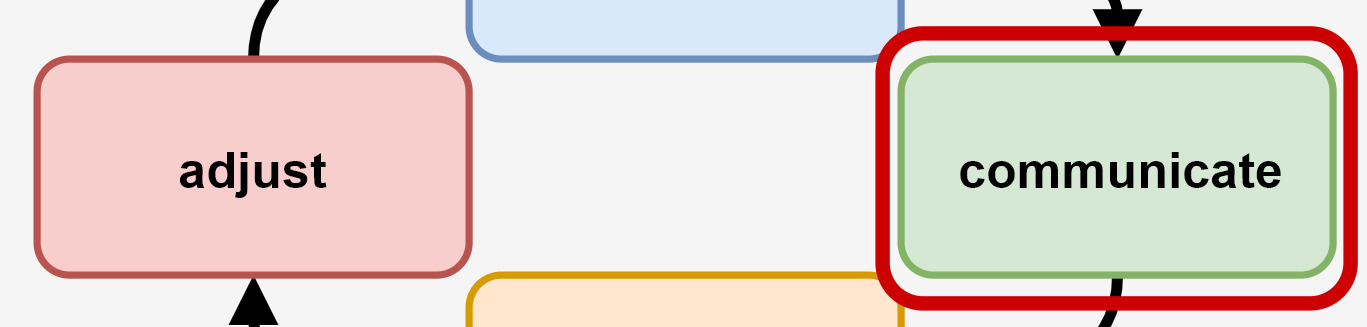
\includegraphics[width=0.75\textwidth]{contents/images/SmartGrazerSectionCommunicate}
	\caption{SmartGrazer: Auszug Kommunikationsphase}
	\label{fig:SmartGrazer-sectionCommunicate}
\end{figure}

Die Kommunikation zwischen SmartGrazer und der Webseite findet über \ac{HTTP} bzw. über \ac{HTTPS} statt. In Konfigurationsdateien kann für jeden Test eine Konfiguration hinterlegt werden. Implementiert wurden die \ac{HTTP}-Methoden \gls{GET} und \gls{POST}, sowie das Übermitteln des Payloads über Cookies.

Zusätzlich besteht die Möglichkeit, eine weitere Aktion, d.h. einen Request, an das SUT zu senden, um sich beispielsweise einzuloggen. Dies wird mittels einer Vorbedingungsaktion ``precondition'' realisiert. Ein Beispiel mit verschiedenen Parametertypen und Vorbedingungen ist im Anhang \ref{lst:full-sut-config} zu finden.

\subsection{SUT-Konfigurationsdatei}
Ein Minimalbeispiel einer solchen SUT-Konfiguration ist in Quelltextbeispiel \ref{lst:minimal-example-SUT} aufgeführt. Jede SUT-Konfiguration hat als Wurzelknoten den Schlüssel ``runconfig'', gefolgt von einer Konfiguration für einen validen Durchlauf. Der valide Durchlauf dient der Applikation als Basis, um später gesendete Payloads zu ermitteln und vergleichen zu können. Im gezeigten Beispiel ist eine Konfiguration für die Google-Suche gegeben. Im Parameter target wird die \ac{URL} des SUT angegeben. Weitere Parameter vom Typ GET und POST, sowie Cookies können unter dem Punkt ``params'' entsprechend hinzugefügt werden.

\begin{lstlisting}[caption={SmartGrazer: Grundaufbau einer SUT-Konfigurationsdatei},label=lst:minimal-example-SUT]
{
  "runconfig": {
    "valid": {
      "action": {
      "filesuffix": "valid",
      "target": "https://www.google.de/search",
      "params": {
        "get": {
          "q": "PAYLOAD"
        }
      }
    },
    "PAYLOAD": "#smartgrazer"
  },
  "attack": {
    "action": {
      "filesuffix": "attack",
      "target": "https://www.google.de/search",
        "params": {
          "get": {
            "q": "PAYLOAD"
          }
        }
} } } }
\end{lstlisting}


\FloatBarrier